\chapter{Free Body Diagrams}


\begin{Exercise}[title = {Blocks on a Table}, label = block1]
[This exercise was originally presented as a free-response question on the 2015 AP Physics 1 exam.] Two blocks are connected with a string and two pulleys over a table, as shown in the figure. Block 1 has a mass of 3 kg and Block 2 has a mass of 9 kg. The blocks are released from rest. Treat the string as massless and the pulleys as massless and frictionless when answering the questions below. 

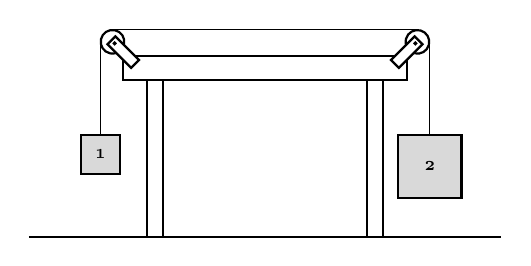
\begin{tikzpicture}
        \draw[thick] (-3, 0) -- (3, 0);
        \draw[thick] (-1.5, 0) rectangle (-1.3, 2);
        \draw[thick] (1.5, 0) rectangle (1.3, 2);
        \draw[thick] (-1.8, 2) rectangle (1.8, 2.3);
        \draw[draw = black, thick, fill=white] (-1.7, 2.15) -- (-1.6, 2.25) -- (-1.9, 2.55) -- (-2, 2.45) -- cycle; 
        \draw[draw=black, thick, fill=white] (1.7, 2.15) -- (1.6, 2.25) -- (1.9, 2.55) -- (2, 2.45) -- cycle;
        \draw[thick, fill=black] (-1.91, 2.46) circle (0.1mm);
        \draw[thick] (-1.79, 2.45) arc (-12:285:0.15);
        \draw[thick, fill=black] (1.91, 2.46) circle (0.1mm);
        \draw[thick] (1.897, 2.335) arc (-105:192:0.15);
        \draw[thin] (-1.94, 2.6382) -- (1.94, 2.6382);
        \draw[thin] (-2.0935, 2.49) -- (-2.0935, 1.3);
        \draw[thin] (2.0927, 2.49) -- (2.0927, 1.3);
        \draw[thick, draw = black, fill = gray!30] (-2.34, 1.3) rectangle (-1.84, 0.8);
        \node[font = \tiny] at (-2.09, 1.05) {\textbf{1}};
        \draw[thick, draw = black, fill = gray!30] (1.69, 1.3) rectangle (2.4954, 0.4946);
        \node[font = \tiny] at (2.0927, 0.8973) {\textbf{2}};
    \end{tikzpicture}
    
\begin{enumerate}
\item Draw free body diagrams for both blocks. Correctly show the relative magnitude of the forces using the relative lengths of the vectors. 
\item Before doing any calculations, describe each block's acceleration as (a) positive or negative, (b) having a magnitude greater or less than \textit{g}. Take the upward direction as positive. 
\item Calculate the acceleration of each block. Take the upward direction as positive and express your answer in terms of \textit{g}. 
\end{enumerate}
\end{Exercise}

\begin{Answer}[ref = block1]
\begin{enumerate}
    \item Each block is acted on by gravity and the tension of the string. The force of gravity on block 2 is 3 times that of block 1, and the tension vector should be between the lengths of the gravity vectors:
    \begin{center}
        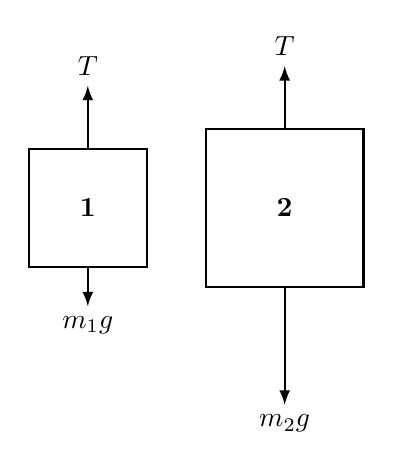
\begin{tikzpicture}
            \draw[thick] (-2, 1) rectangle (-0.5, -0.5);
            \draw[thick] (2.25, 1.25) rectangle (0.25, -0.75);
            \node[] at (-1.25, 0.25) {\textbf{1}};
            \node[] at (1.25, 0.25) {\textbf{2}};
            \draw[thick, -latex] (-1.25, -0.5) -- (-1.25, -1) node[below] {$m_1g$};
            \draw[thick, -latex] (-1.25, 1) -- (-1.25, 1.8) node[above] {$T$};
            \draw[thick, -latex] (1.25, -0.75) -- (1.25, -2.25) node[below] {$m_2g$};
            \draw[thick, -latex] (1.25, 1.25) -- (1.25, 2.05) node[above] {$T$};
        \end{tikzpicture}
    \end{center}

    \item Block 1 will have a positive acceleration with a magnitude less than \textit{g}. Block 2 will have a negative acceleration with a magnitude greater than \textit{g}.

    \item Since the blocks are connected, they will move as a system and therefore have the same magnitude acceleration. From this, the free body diagrams, and Newton's Second Law, we know that:
    $$m_1 a  = T - m_1 g$$
    $$m_2 \left( - a \right) = T - m_2 g$$

    We know $m_1$ and $m_2$, so the two unknowns are $T$ and $a$. One way to solve this system of equations would be to subtract equation 2 from equation 1:
    $$m_1 a + m_2 a = m_2 g - m_1 g$$
    $$a = \frac{m_2 - m_1}{m_1 + m_2} g$$

    Substituting for the masses, we see that:
    $$a = \frac{9 - 3}{9 + 3}g = \frac{6}{12}g = \frac{1}{2}g$$

    Therefore, Block 1 is accelerating at $+\frac{1}{2}g$ and Block 2 is accelerating at $-\frac{1}{2}g$.
\end{enumerate}
\end{Answer}

Now here's an interesting question: what happens if we add another mass to the system? Imagine that a third block with a mass of 15 kg is laid on the table from the previous exercise and the string is attached to each side, as shown below. 
\begin{center}
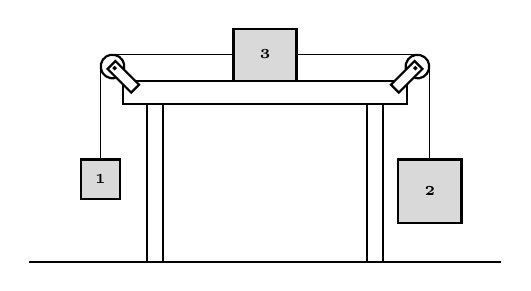
\begin{tikzpicture}
        \draw[thick] (-3, 0) -- (3, 0);
        \draw[thick] (-1.5, 0) rectangle (-1.3, 2);
        \draw[thick] (1.5, 0) rectangle (1.3, 2);
        \draw[thick] (-1.8, 2) rectangle (1.8, 2.3);
        \draw[draw = black, thick, fill=white] (-1.7, 2.15) -- (-1.6, 2.25) -- (-1.9, 2.55) -- (-2, 2.45) -- cycle; 
        \draw[draw=black, thick, fill=white] (1.7, 2.15) -- (1.6, 2.25) -- (1.9, 2.55) -- (2, 2.45) -- cycle;
        \draw[thick, fill=black] (-1.91, 2.46) circle (0.1mm);
        \draw[thick] (-1.79, 2.45) arc (-12:285:0.15);
        \draw[thick, fill=black] (1.91, 2.46) circle (0.1mm);
        \draw[thick] (1.897, 2.335) arc (-105:192:0.15);
        \draw[thin] (-1.94, 2.6382) -- (1.94, 2.6382);
        \draw[thin] (-2.0935, 2.49) -- (-2.0935, 1.3);
        \draw[thin] (2.0927, 2.49) -- (2.0927, 1.3);
        \draw[thick, draw = black, fill = gray!30] (-2.34, 1.3) rectangle (-1.84, 0.8);
        \node[font = \tiny] at (-2.09, 1.05) {\textbf{1}};
        \draw[thick, draw = black, fill = gray!30] (1.69, 1.3) rectangle (2.4954, 0.4946);
        \node[font = \tiny] at (2.0927, 0.8973) {\textbf{2}};
        \draw[thick, draw = black, fill = gray!30] (-0.4, 2.3) rectangle (0.4, 2.96);
        \node[font = \tiny] at (0, 2.638) {\textbf{3}};
    \end{tikzpicture}
\end{center}

compare re-doing all the fbds to thinking about the entire system

